\documentclass[12pt]{report}
\usepackage{mathptmx}
\usepackage[left=2.5cm, right=2.5cm, top=2.5cm, bottom=2.5cm]{geometry}
\usepackage[slovak]{babel}
\usepackage{pdfpages}
\usepackage{array}
\usepackage{tabularx}
\linespread{1.0} 
\renewcommand{\arraystretch}{1.5}
\newcommand{\mytablewidth}{\textwidth}
\author{Mykyta Fedorin}
\title{BikeXpress}
\date{}

\begin{document}

\maketitle

\chapter{Použivateľská špecifikácia}
\section{Stručný úvod do problematiky}
\subsection{Vseobecny scenar pouzitia}

Firma BikeXpress sa zaoberá požičaním bicyklov a žiada o vytvorenie softvéru prevádzky(ďalej
len Systém). Distribúciu služieb bude robiť pomocou staníc z bicyklami, ktore umiestni po celej
Bratislave. Každá stanica bude obsahovať hlavný riadiaci prístroj. Tento prístroj bude riadiť za-
mok, pomocou ktorého je uzamknuty každý z bicyklov v danej stanici. Systém mal by umožniť
zákazníkom používať platené služby pozicania bicyklov firmy BikeXpress. Služby budú pozostávať
z plateného pozicania bicykla, s cieľom pomôcť zákazníkovi sa dostať tam, kde potrebuje a vrátiť
bicykel naspäť do bližšej stanice.

Hlavný scenár použitia servisu:

Systém je rozdelený na dve funkčné časti. Prvá časť je určená pre majiteľa (správcu) služby bike
sharing a druhá pre ľudí (zákazníkov), ktorí chcú využívať bicykle správcu na vlastnú prepravu po
meste. Správca ma úplnú kontrolu nad celým systémom, t.j. vidí všetky servisné dáta pre konkrétny
bicykel, vie nastavovať HW aj SW pre každý bicykel zvlášť alebo pre celú skupinu bicyklov a to všetko
vzdialene. 

Tak isto vidí aj štatistiku používania bicyklov. Systém ponúka správcovi definovať rôzne
tarify prispôsobené napr. podľa dátumu a času. V systéme je integrovaný aj mailový klient a SMS brána,
ktoré slúžia na komunikáciu so zákazníkmi a posielaní upozornení alebo informačných správ pre
zákazníkov. Zaujímavou funkciou je aj tzv. servisný modul, ktorý upozorňuje správcu o blížiacich sa
termínoch technickej údržby bicyklov. Napr. po prejdení určitých kilometrov sa musia skontrolovať
brzdy, prehadzovačka, dezén, svetlá. 

Pre zákazníkov je určená webová aplikácia a mobilná aplikácia
(Android, IOS). Ich funkcionalita obsahuje zobrazenie on-line mapy obsadenosti bicyklov a zobrazenie
mapy staníc bike sharing-u. Každý zákazník má svoj používateľský profil, kde vidí svoje štatistiky
a históriu vypožičaní a platieb. Tak isto sa zákazníkovi zobrazujú v profile aj rôzne akcie a zľavy,
ktorých odber si môže aktivovať alebo zablokovať. Aplikácia vie vykonať bezpečnú online platbu.
Mobilná aplikácia dokáže to isté ako webová, ale naviac má podporu pre rýchle vypožičanie pomocou
NFC/snímania čiarového alebo QR kódu, ďalej obsahuje navigáciu k najbližšej stanici bike sharing-u
(keďže sa predpokladá, že telefón má GPS modul).

\subsection{Casti systemu}
\begin{enumerate}
    \item Webova stranka
    \item Mobilna aplikacia
    \item Softver pre stanice
    \item Administratorské konto
\end{enumerate}
 
\section{Pouzivatelske poziadavky}
\subsection{Funkcionalne poziadavky}

Webová stránka a mobilná aplikácia musia mať nasledovnú funkcionalitu:

\begin{enumerate}
    \item Registrácia používateľa \\
        Používateľ musí byť schopný si vytvoriť konto. Po skončení registracie 
        aplikacia musí upozorniť použivateľa, či sa podarilo konto vytvoriť.
        Na vytvorenie konta stači zadať mailovu adresu a vymyslieť si heslo.
        
    \item Zobrazenie konta používateľa \\
        Aplikácia musí byt schopná zobraziť históriu platieb a štatistík používania 
        bicyklov. 

    \item Zobrazenie mapy staníc \\
        Mapa staníc musí zobrazovať všetky dostupné stanice v meste používateľa. 
        Každá jednotlivá stanica musí mať informácie o počte dostupných bicyklov.
        
    \item Platba za služby \\
        Táto funkcia umožní používateľom zaplatiť za služby servisu zadáním údajov platobnej karty.
        
    \item Rezervácia bicykla \\
        Poživateľ musi byť schopný objednať si bicykel na konkrétnej stanici.

\end{enumerate}

Navyše, mobilná aplikácia musí byť schopná:

\begin{enumerate}
    \item Skenovať QR-kód \\
        Používateľ musí byť schopný dostať sa k rezervovanému bicyklu skenovaním QR kódu na bicykli.
        
    \item Skenovať NFC čip \\
        Používateľ musí byť schopný dostať sa k rezervovanému bicyklu skenovaním NFC čipu na bicykli.
\end{enumerate}

Administratorske konto je určené pre majiteľa prevádzky a musí spĺňať nasledujúcu funkcionalitu:

\begin{enumerate}
    \item Zobrazovať všetky servisné údaje pre konkrétny bicykel \\
        Ide o informácie o dĺžke prevádzky, technickom stave a štatistike používania bicyklov.
        
    \item Umožniť definovanie tarifov \\
        Majiteľ môže definovať sadzby tarifov prostredníctvom administratorského konta.
        
    \item Obsahovať e-mailového klienta a SMS bránu \\
        Pomocou administratorského konta musí majiteľ byť schopný informovať zákazníkov prostredníctvom 
        e-mailových a SMS správ.

\end{enumerate}

\subsection{Nefunkcionalné požiadavky}

\begin{enumerate}
    \item Registracia \\
	      Applikacia musí overiť správnosť tvaru zadanej mailovej adresy podľa RFC 5322 
        a upozorniť používateľa v prípade zle zadanej adresy. Heslo musí obsahovať minimálne 8 
        znakov, minimálne jedno veľké písmeno, minimálne jeden špeciálny znak.

    \item Zobrazenie historie platieb\\
        Ide o zoznam platieb z informaciami o učte z ktoreho prešla platba, datume a vyške poplatku.

    \item Zobrazenie štatistiky použivania bicyklov\\
        To sú informácie o počte prejdenych kilometrov a dĺžke používania bicykla v každej objdenavke.

    \item Bezpečnosť\\
        Prístup k účtu administrátora prevádzky v administratorskom konte nesmie byť indexovaný verejne vo
        vyhľadávacích službách. Webová stránka musí používať šifrovaný protokol HTTPS a POST na odosielanie osobných 
        údajov na server.
\end{enumerate}

\chapter{Systémova špecifikácia}
\section{Diagramy prípadov použitia}
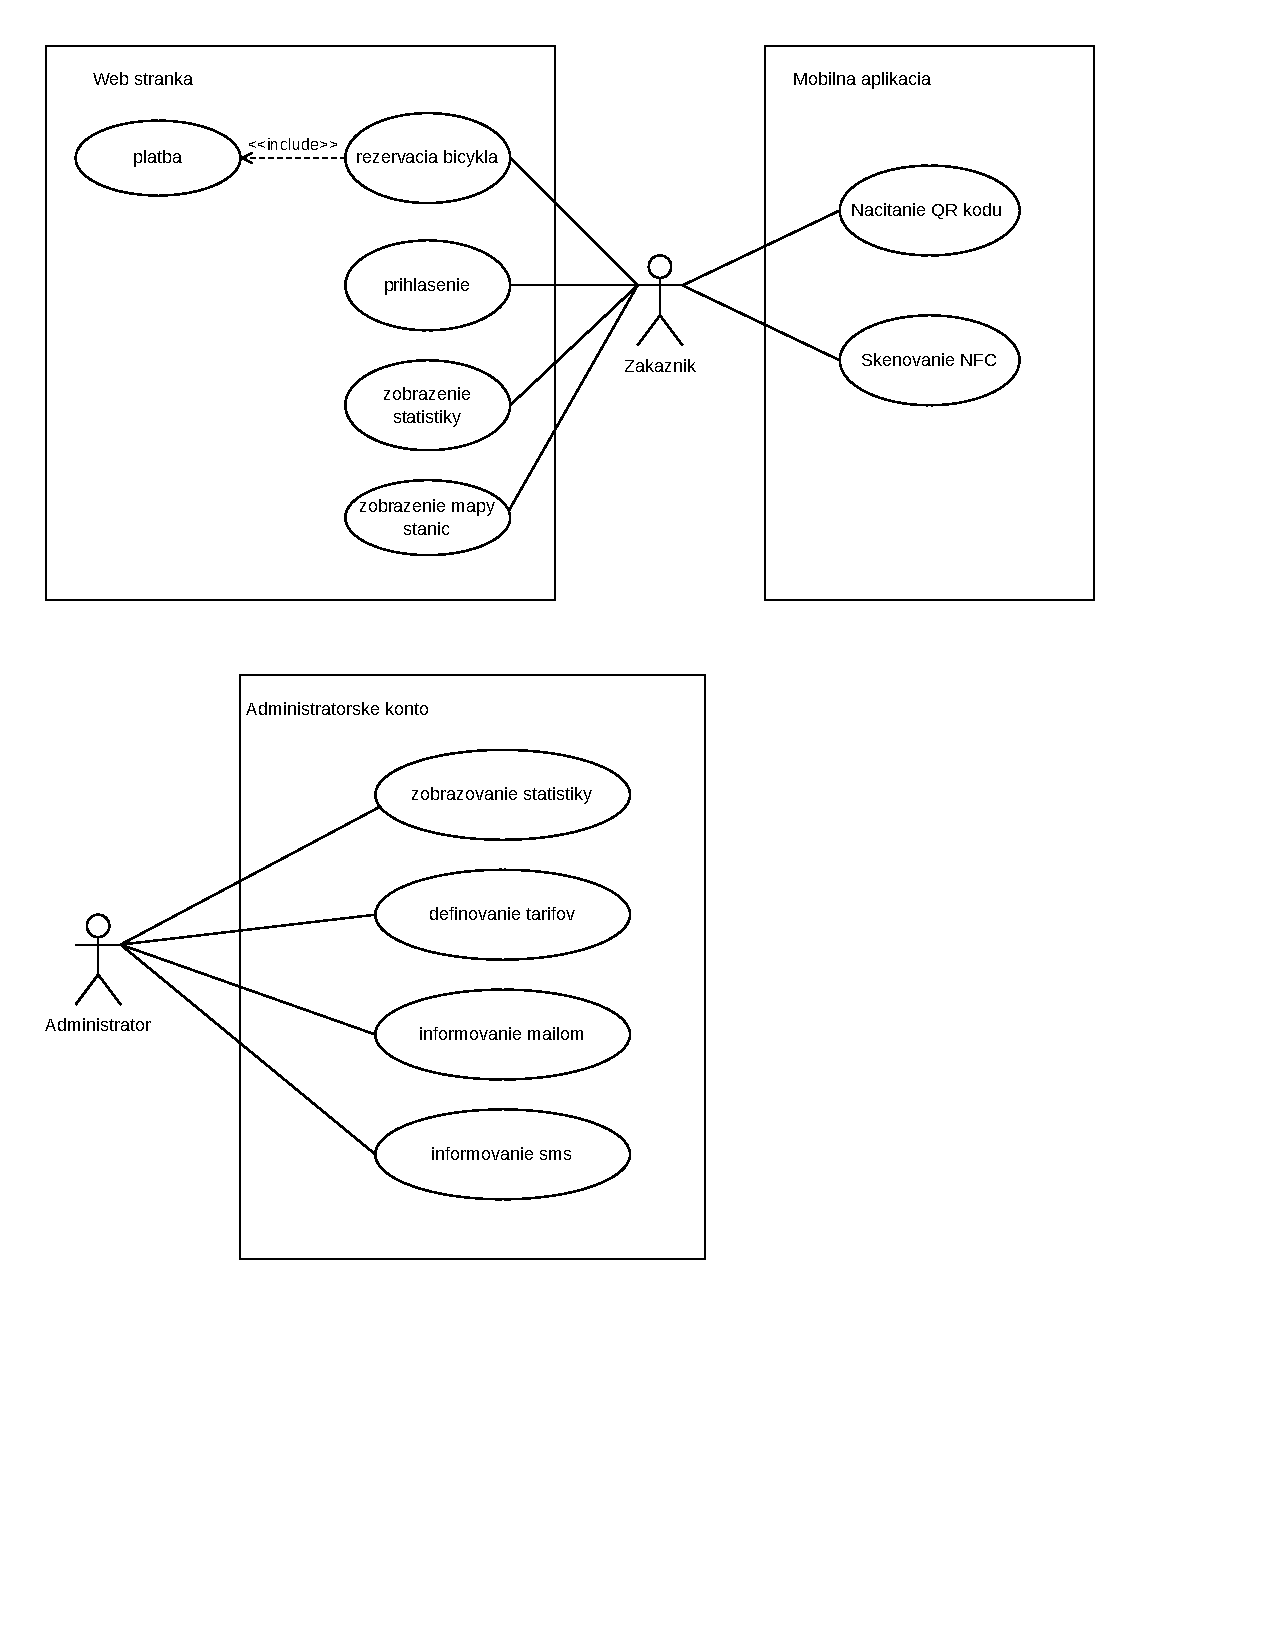
\includepdf[pages=-]{diagrams/pdf/uc.pdf}
\clearpage 

\section{Use case tabluľky}
\begin{table}[h]
  \centering
  \begin{tabular}{|p{12cm}|}
   \hline
   \multicolumn{1}{|c|}{ \textbf{Rezervacia bicykla}} \\
   \hline
   Číslo prípadu použitia: UC1\\
   \hline
   Opis: preberanie bicykla zakaznikom zo stanici.\\
   \hline
   Akteri: Zákaznik\\
   \hline
   Vstupné podmienky: Zákaznik sa authorizuje na stranke.\\
   \hline
   Inicializacia: Aktivuje sa sluzba prehladu stanic.\\
   \hline
   Hlavný scenár:
   \begin{enumerate} 
       \item Webova stranka zobrazi mapu stanic.
       \item Klient si vyberie stanicu.
       \item Webova stranka ukaze zákaznikovi existujuce tarify.
       \item Zákaznik si zvoli tarif. 
       \item Zakazik zaplati tarif zadaním udajov platobnej karty.
       \item Webova stranka vygeneruje číslo a poskytne ho zákaznikovi.
       \item Zákaznik si číslo zada na zvolenej stanici.
       \item Stanica uvoľni bicykel.
   \end{enumerate}\\
   \hline
   Výstupné podmienky: Zákaznik preberie bicykel.\\
   \hline
   Alternatívný scenár 1:
   \begin{enumerate} 
       \item Ak klient nedisponuje dostatkom peňazi, stranka proces
             platby zruši a nevygeneruje ziadne číslo. 
       \item Klient si zvolí iný tarif a tok pokračuje bodom 5 hlavneho scenara.
   \end{enumerate}\\
   \hline
   Alternatívný scenár 2:
   \begin{enumerate} 
       \item Ak na vybranej stanici nie su volne bicykle, webova stranka 
             upozorni na to pouzivatela. 
       \item Klient si zvoli inu stanicu a tok pokračuje bodom 3 hlavneho scenara.
   \end{enumerate}\\
   \hline
  \end{tabular}
  \caption{Preberanie zákaznikom bicykla}
  \label{tab:use_case_steps}
\end{table}

\clearpage 

\begin{table}[h]
  \centering
  \begin{tabular}{|p{12cm}|}
   \hline
   \multicolumn{1}{|c|}{ \textbf{Definovanie tarifov}} \\
   \hline
   Číslo prípadu použitia: UC2\\
   \hline
   Opis: Administrator musi byt schopny zadefinovat novy tarif alebo upravit stare.\\
   \hline
   Akteri: Administrator BikeXpress\\
   \hline
   Vstupné podmienky: Administrator je prihlaseny pod učtom s príslušnými pravami.\\
   \hline
   Inicializacia: Administrator aktivuje službu definovania a prehľadu jednotlivych tarifov.\\
   \hline
   Hlavný scenár:
   \begin{enumerate} 
       \item Webova stranka zobrazi existujuce tarify.
       \item Administrator si zvoli vytvorit nový tarif. 
       \item Administrator vyplni poskytnuty systemom formular.
       \item Stranka ulozi novu polozku do databazy.
   \end{enumerate}\\
   \hline
   Výstupné podmienky: Obnovi sa zoznam alebo stav tarifov.\\
   \hline
   Alternatívný scenár 1:
   \begin{enumerate} 
       \item Ak zadane data nie su vo vhodnom tvare, stranka upozorni na to administratora.
       \item Administrator si data upravi a tok pokracuje bodom 4 hlavneho scenara.
   \end{enumerate}\\
   \hline
   Alternatívný scenár 2:
   \begin{enumerate} 
       \item Administrator si zvoli zmenit existujuce tarify.
       \item Stranka zobrazi uz existujuci tarif a umozni ho upravu.
       \item Administrator upravi prislusne tarify a system ulozi ich do databazy.
   \end{enumerate}\\
   \hline
  \end{tabular}
  \caption{Definovanie tarifov v systeme}
  \label{tab:use_case_steps}
\end{table}


\clearpage 

\begin{table}[h]
  \centering
  \begin{tabular}{|p{12cm}|}
   \hline
   \multicolumn{1}{|c|}{ \textbf{Nacitanie QR kodu}} \\
   \hline
   Číslo prípadu použitia: UC3\\
   \hline
   Opis: Zakaznik nacita QR kod bicykla, zaplati a dostane bicykel\\
   \hline
   Akteri: Zakaznik\\
   \hline
   Vstupné podmienky: Zakaznik je prihlaseny.\\
   \hline
   Inicializacia: Zakaznik aktivuje funkciu nacitavania QR kodu v aplikacii.\\
   \hline
   Hlavný scenár:
   \begin{enumerate} 
       \item Aplikacia pozaduje snimanie QR kodu.
       \item Zakaznik QR kod nacita. 
       \item Aplikacia ukaze zákaznikovi existujuce tarify.
       \item Zákaznik si zvoli tarif. 
       \item Zakazik zaplati tarif zadaním udajov platobnej karty.
       \item Stanica uvolni bicykel
   \end{enumerate}\\
   \hline
   Výstupné podmienky: Zakaznik preberie bicykel.\\
   \hline
   Alternatívný scenár 1:
   \begin{enumerate} 
       \item Ked zakaznik nacita neplatny QR kod, aplikacia upozorni ho 
             o tom.
       \item Zakaznik nacita spravny QR kod a tok pokracuje bodom 3 hlavneho scenara.
   \end{enumerate}\\
   \hline
   Alternatívný scenár 2:
   \begin{enumerate} 
       \item Ak klient nedisponuje dostatkom peňazi, aplikacia proces
             platby zruši. 
       \item Klient si zvolí iný tarif a tok pokračuje bodom 5 hlavneho scenara.
   \end{enumerate}\\
   \hline
  \end{tabular}
  \caption{Preberanie bicykla pomocou QR kodu}
  \label{tab:use_case_steps}
\end{table}


\clearpage 

\section{Diagram tried}
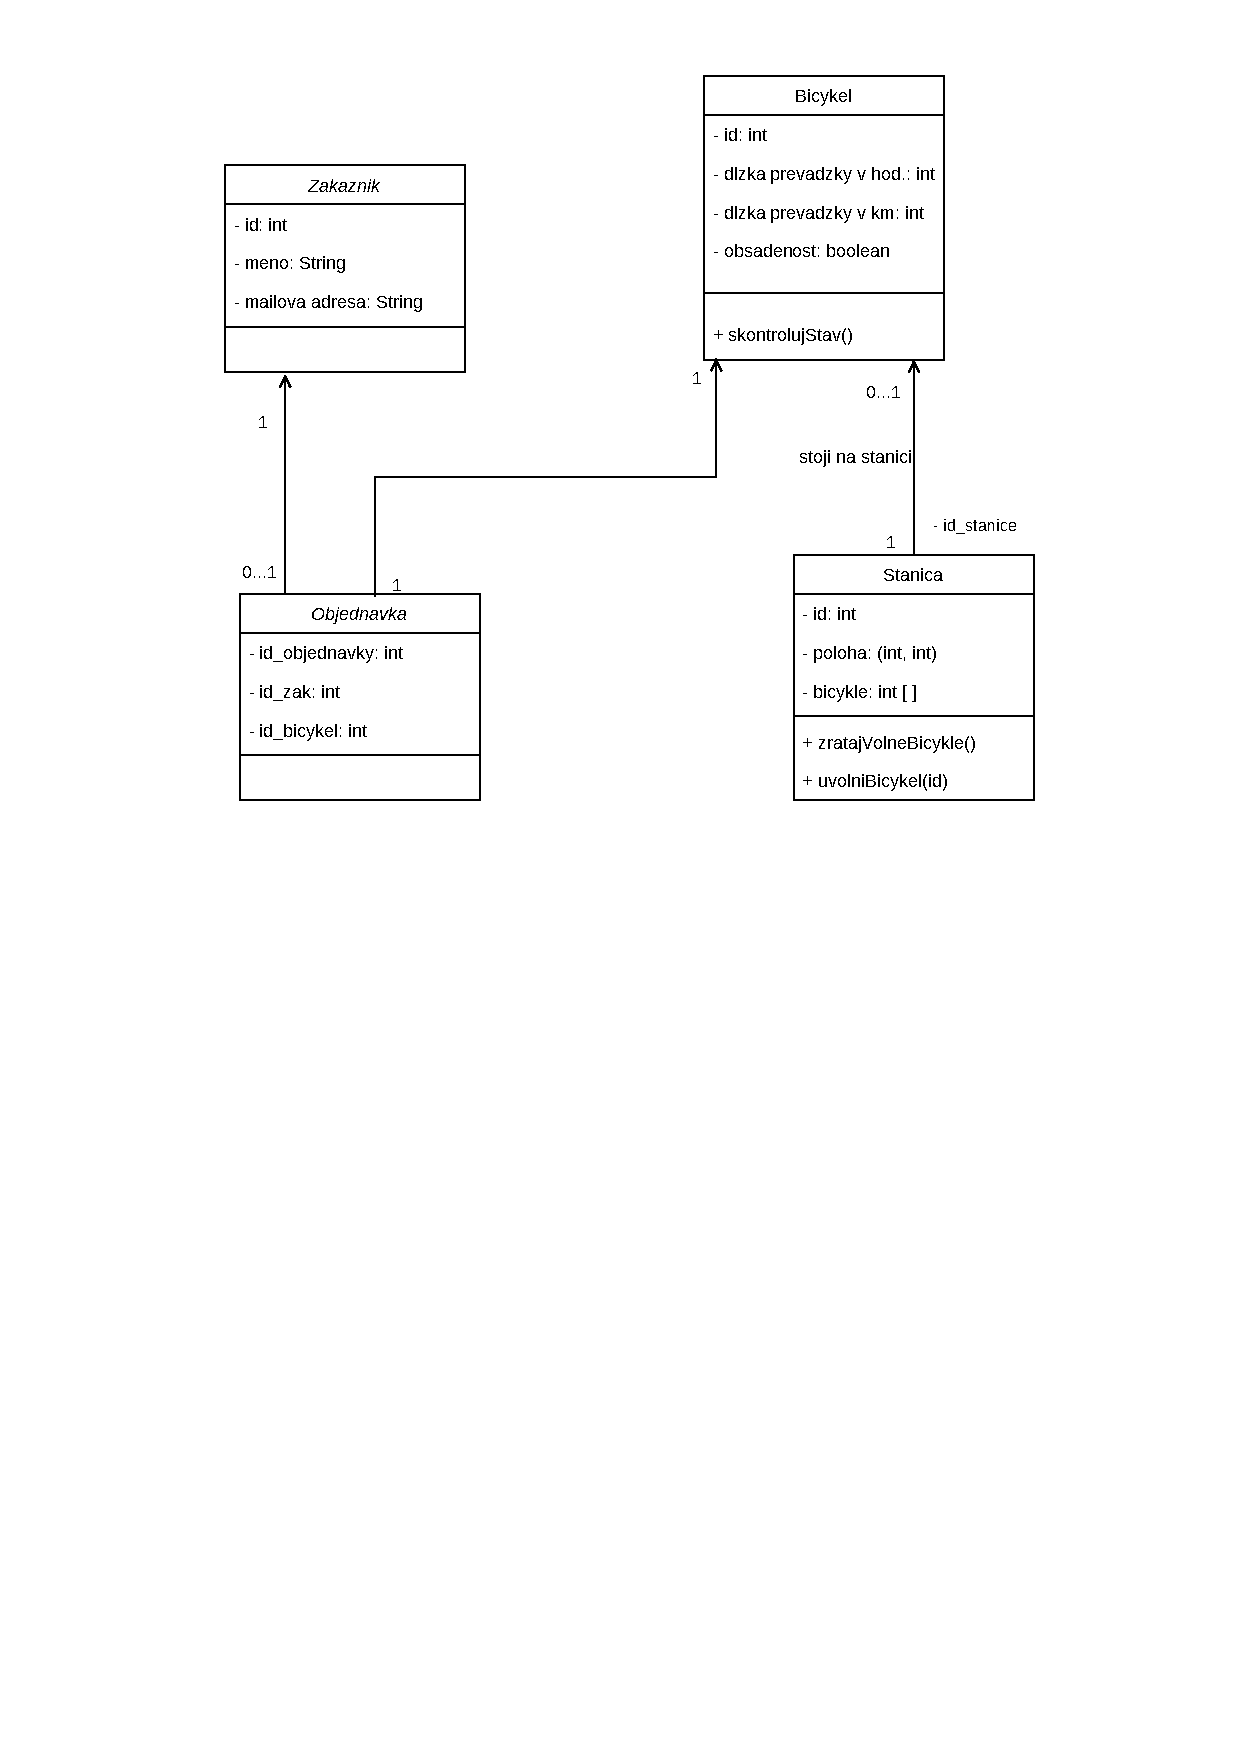
\includepdf[pages=-]{diagrams/pdf/class.pdf}
\clearpage 

\section{Diagramy aktivit a sekvencne diagramy}
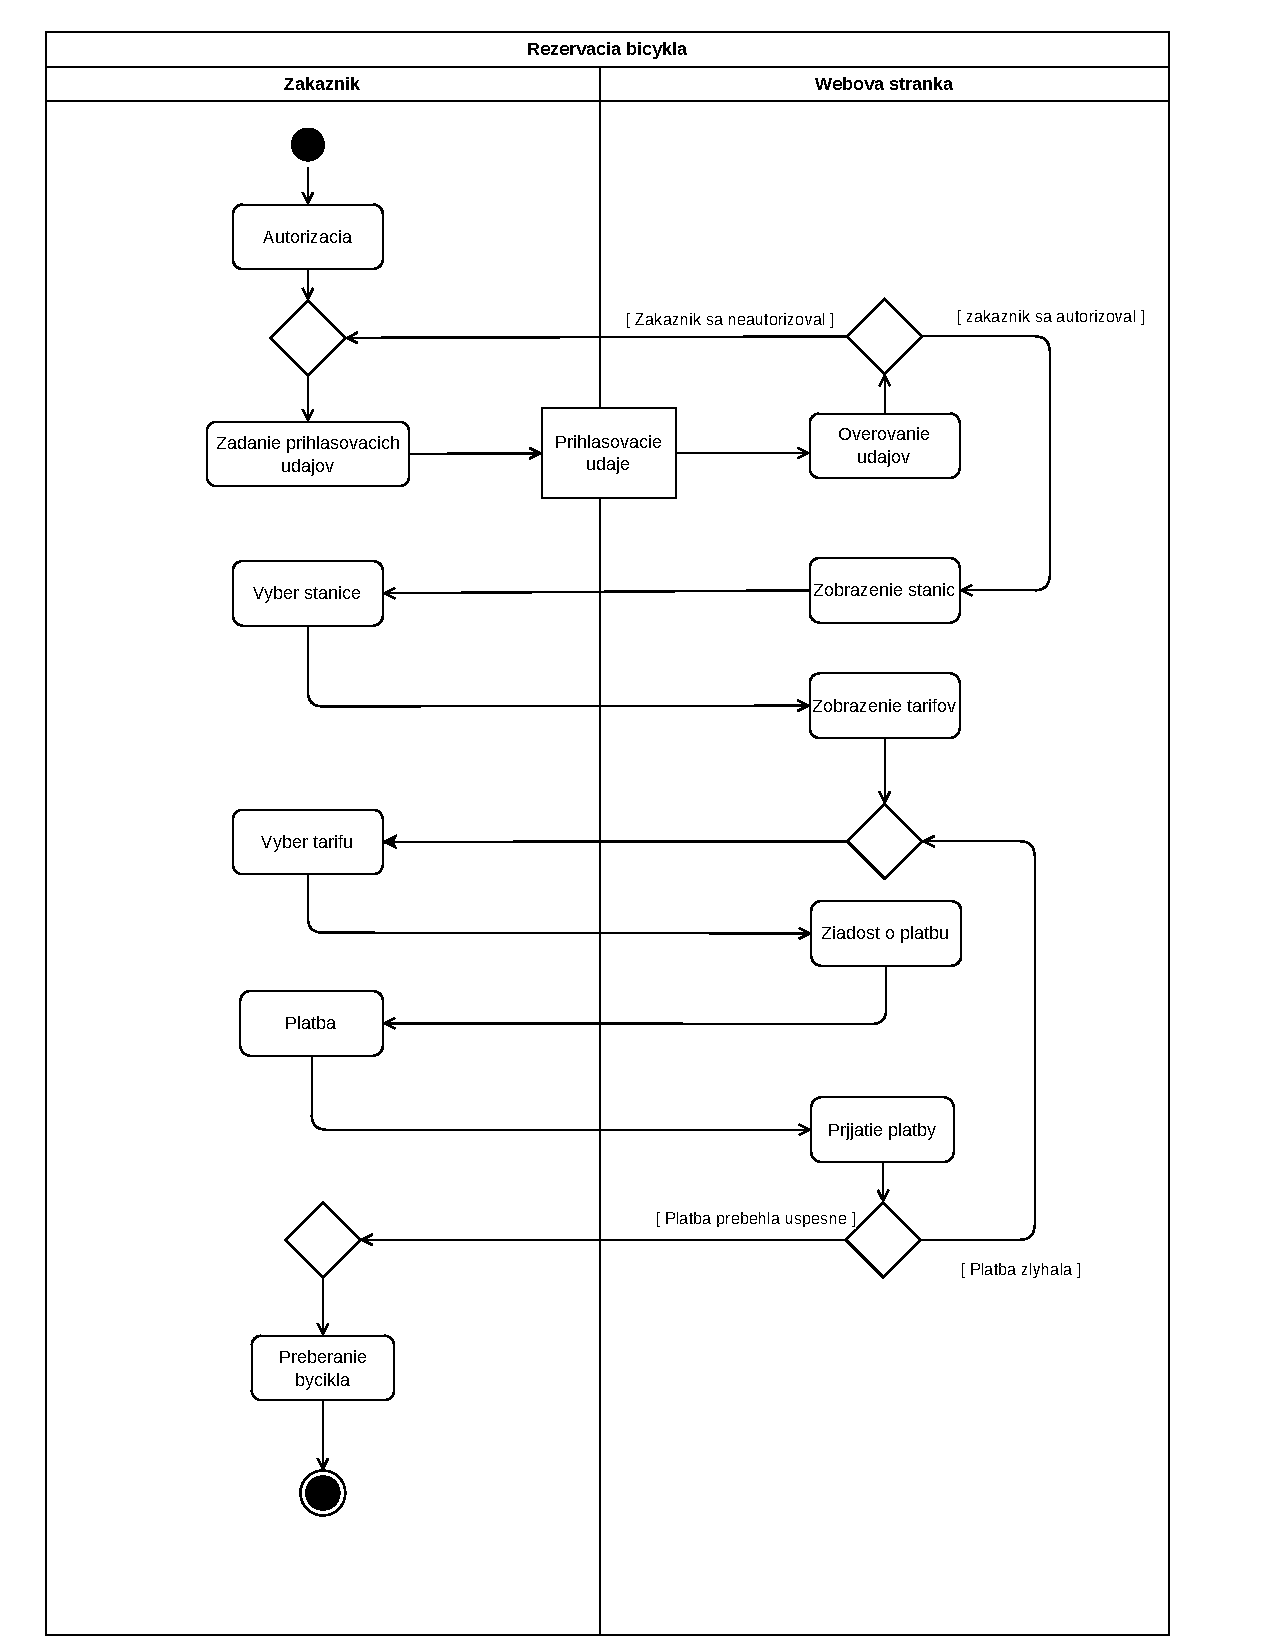
\includepdf[pages=-]{diagrams/pdf/activity.pdf}
\clearpage 

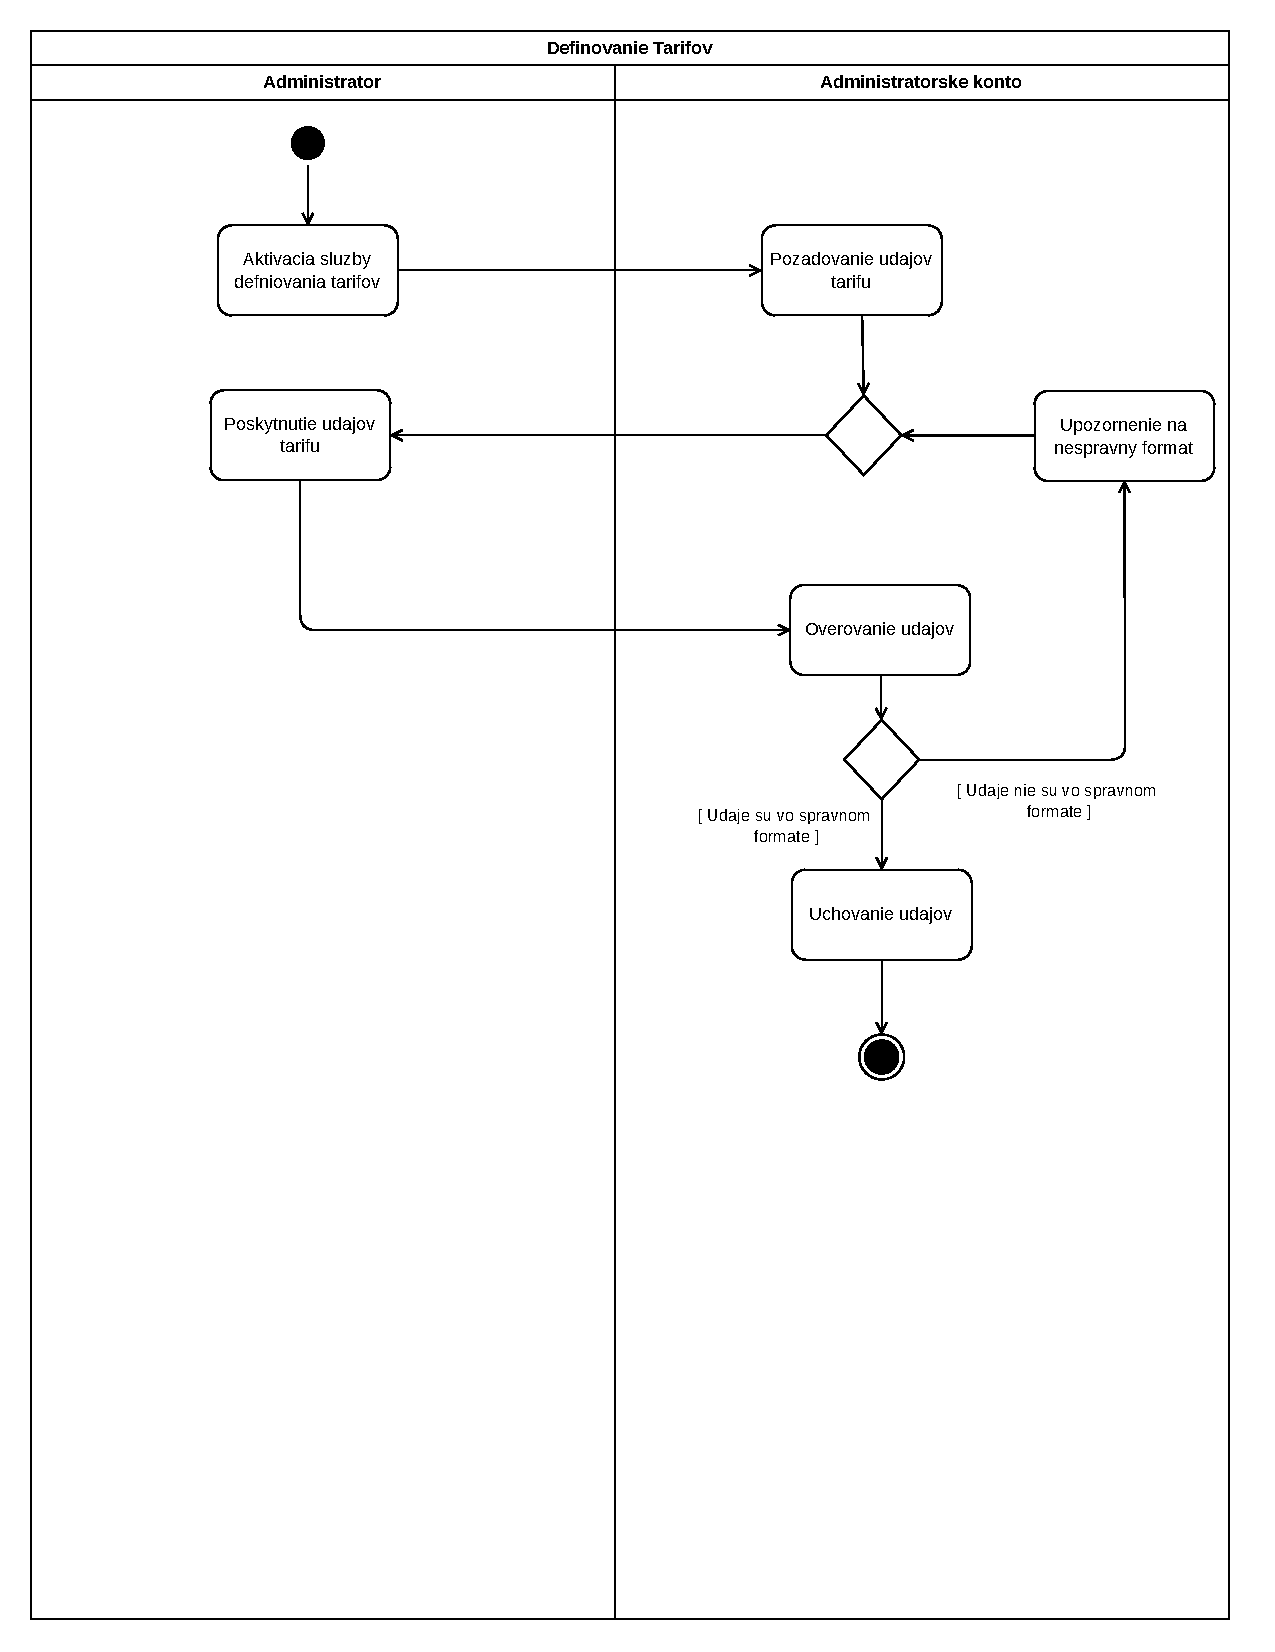
\includepdf[pages=-]{diagrams/pdf/activity2.pdf}
\clearpage 

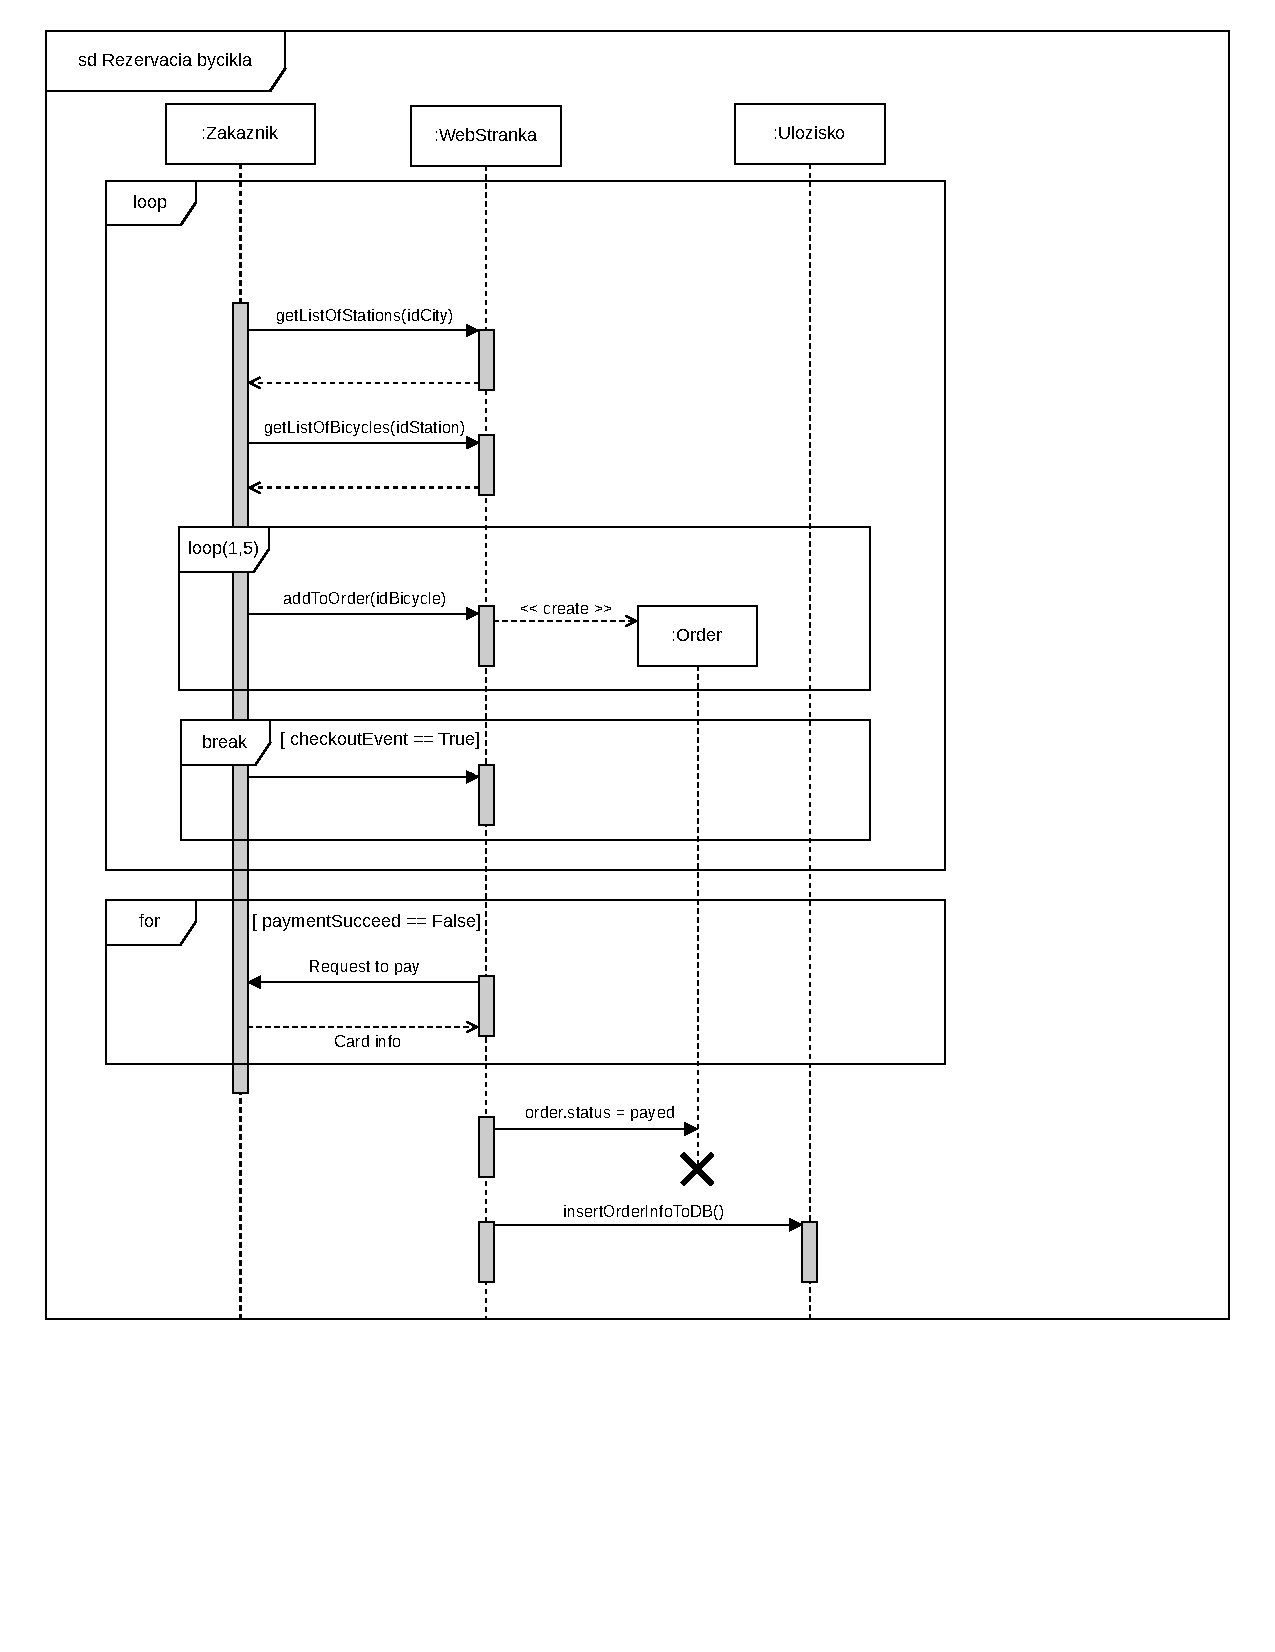
\includepdf[pages=-]{diagrams/pdf/sequence.pdf}
\clearpage 

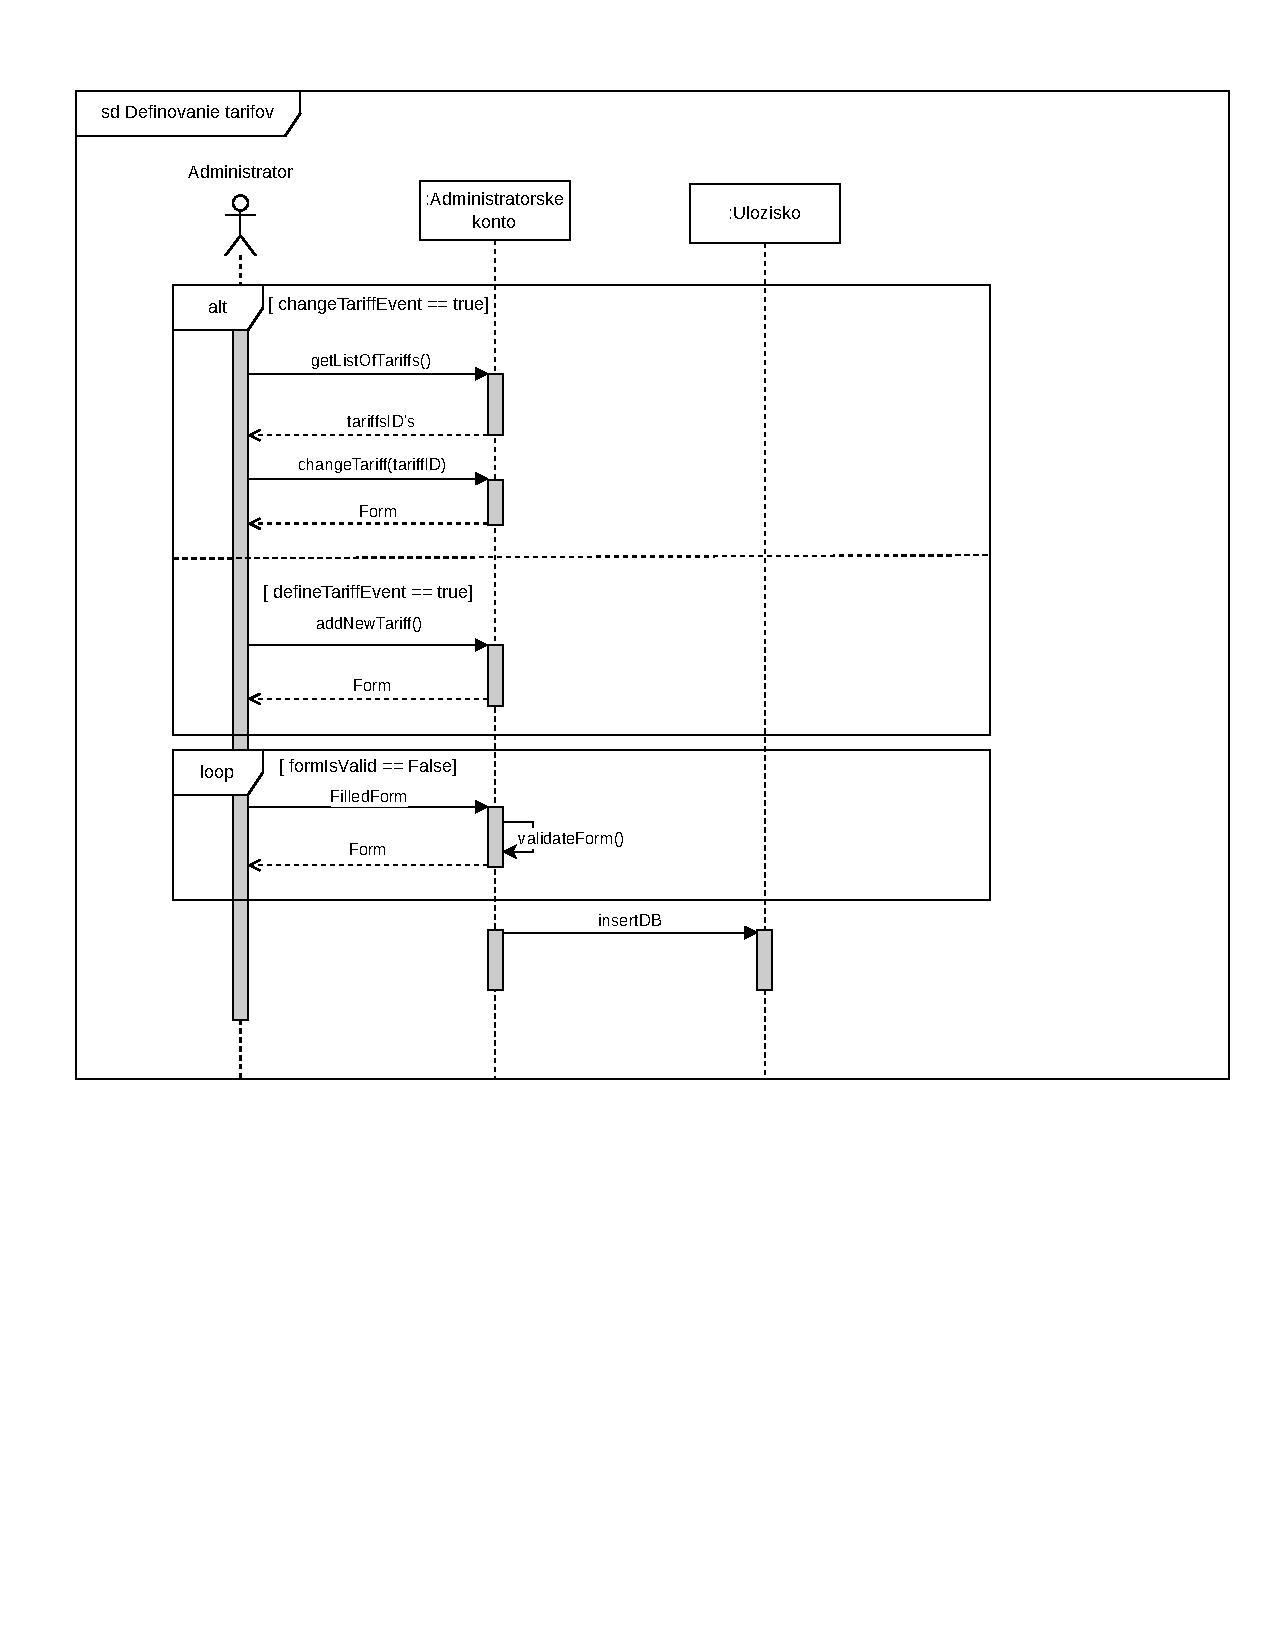
\includepdf[pages=-]{diagrams/pdf/sequence1.pdf}

\chapter{Akceptačné testy}
\begin{table}[h]
  \centering
  \begin{tabularx}{\mytablewidth}{|c|c|c|X|} 
      \hline 
      \textbf{ID} & 1 & \textbf{Názov} & Zobrazenie mapy stanic 
  \end{tabularx}

  \begin{tabularx}{\mytablewidth}{|c|c|c|X|} 
      \hline 
      \textbf{Prípad pouzitia} & UC1 & \textbf{Úroveň splnenia testu} & Musi
  \end{tabularx}

  \begin{tabularx}{\mytablewidth}{|c|X|} 
      \hline 
      \textbf{Rozhranie} & pouzivatel
  \end{tabularx}

  \begin{tabularx}{\mytablewidth}{|c|X|} 
      \hline 
      \textbf{Ucel} & Overenie spravnej funkcnosti zobrazenia mapy stanic
  \end{tabularx}

  \begin{tabularx}{\mytablewidth}{|c|X|} 
      \hline 
      \textbf{Vstupne podmienky} & Pouzivatel aktivoval funkciu zobrazenia mapy stanic
  \end{tabularx}

  \begin{tabularx}{\mytablewidth}{|c|X|} 
      \hline 
      \textbf{Vystupne podmienky} & Web stranka zobrazi interaktivnu mapu s vyznacenymi stanicami,
      kazda z ktorych obsahuje informacie o pocte volnych byciklov.
  \end{tabularx}

  \begin{tabularx}{\mytablewidth}{|p{2em}|X|X|X|} 
      \hline 
      \textbf{Krok} & \textbf{Akcia} & \textbf{Ocakavana reakcia} & \textbf{Skutocna reakcia}
  \end{tabularx}

  \begin{tabularx}{\mytablewidth}{|p{2em}|X|X|X|} 
      \hline 
      1 & 
      Volba zobrazenia mapy stanic & 
      Zobrazi sa interaktivna mapa stanic & 
      Zobrazuje sa mapa, ale stanice nie su vyznacene
  \end{tabularx}
  \begin{tabularx}{\mytablewidth}{|p{2em}|X|X|X|} 
      \hline 
      2 & 
      Posun mapy pomocou kurzora & 
      Mapa sa posunie a zobrazi dalsi region & 
      Mapa sa neposuva
  \end{tabularx}
  \begin{tabularx}{\mytablewidth}{|p{2em}|X|X|X|} 
      \hline 
      3 & 
      Kliknutie na znacku stanice & 
      Zobrazi sa informacie o stanice & 
      Informacie sa zobrazuju, ale nie su skutocne
  \end{tabularx}
  \begin{tabularx}{\mytablewidth}{|X|} 
      \hline
  \end{tabularx}
\end{table}

\begin{table}[h]
  \centering
  \begin{tabularx}{\mytablewidth}{|c|c|c|X|} 
      \hline 
      \textbf{ID} & 2 & \textbf{Názov} & Rezervacia bycikla
  \end{tabularx}

  \begin{tabularx}{\mytablewidth}{|c|c|c|X|} 
      \hline 
      \textbf{Prípad pouzitia} & UC1 & \textbf{Úroveň splnenia testu} & Musi
  \end{tabularx}

  \begin{tabularx}{\mytablewidth}{|c|X|} 
      \hline 
      \textbf{Rozhranie} & pouzivatel
  \end{tabularx}

  \begin{tabularx}{\mytablewidth}{|c|X|} 
      \hline 
      \textbf{Ucel} & Overenie spravnej funkcnosti rezervacii byciklov
  \end{tabularx}

  \begin{tabularx}{\mytablewidth}{|c|X|} 
      \hline 
      \textbf{Vstupne podmienky} & Pouzivatel sa autorizoval, vybral stanicu a zvolil si zaplatit za bycikel
  \end{tabularx}

  \begin{tabularx}{\mytablewidth}{|c|X|} 
      \hline 
      \textbf{Vystupne podmienky} & Pouzivatel zaplatil sumu tarifu a dostal bycikel
  \end{tabularx}

  \begin{tabularx}{\mytablewidth}{|p{2em}|X|X|X|} 
      \hline 
      \textbf{Krok} & \textbf{Akcia} & \textbf{Ocakavana reakcia} & \textbf{Skutocna reakcia}
  \end{tabularx}

  \begin{tabularx}{\mytablewidth}{|p{2em}|X|X|X|} 
      \hline 
      1 & 
      Pouzivatel zvolil stanicu a poziadal o rezervaciu & 
      Stranka vypise zoznam tarifov s moznostou vyberu a platby & 
      Stranka vypisala zoznam tarifov s moznostou vyberu a platby 
  \end{tabularx}
  \begin{tabularx}{\mytablewidth}{|p{2em}|X|X|X|} 
      \hline 
      2 & 
      Pouzivatel si zvolil tarif a chce ho zaplatit & 
      Zobrazil sa formular na zadanie udajov platobnej karty& 
      Zobrazil sa formular na zadanie udajov platobnej karty
  \end{tabularx}
  \begin{tabularx}{\mytablewidth}{|p{2em}|X|X|X|} 
      \hline 
      3 & 
      Pouzivatel zadal udaje karty v nespravnom tvare& 
      Stranka upozorni pouzivatela o nespravnom vstupe & 
      Stranka uspesne spracuje transakciu
  \end{tabularx}
  \begin{tabularx}{\mytablewidth}{|X|} 
      \hline
  \end{tabularx}
\end{table}



\begin{table}[h]
  \centering
  \begin{tabularx}{\mytablewidth}{|c|c|c|X|} 
      \hline 
      \textbf{ID} & 3 & \textbf{Názov} & Definovanie tarifov
  \end{tabularx}

  \begin{tabularx}{\mytablewidth}{|c|c|c|X|} 
      \hline 
      \textbf{Prípad pouzitia} & UC2 & \textbf{Úroveň splnenia testu} & Musi
  \end{tabularx}

  \begin{tabularx}{\mytablewidth}{|c|X|} 
      \hline 
      \textbf{Rozhranie} & Administrator
  \end{tabularx}

  \begin{tabularx}{\mytablewidth}{|c|X|} 
      \hline 
      \textbf{Ucel} & Overenie spravnej funkcnosti definovania tarifov
  \end{tabularx}

  \begin{tabularx}{\mytablewidth}{|c|X|} 
      \hline 
      \textbf{Vstupne podmienky} & Pouzivatel je prihlaseny pod administratorskym kontom a 
                                   a aktivoval sluzbu definovania tarifov
  \end{tabularx}

  \begin{tabularx}{\mytablewidth}{|c|X|} 
      \hline 
      \textbf{Vystupne podmienky} & V databaze je ulozeny aktualizovany zoznam tarifov
  \end{tabularx}

  \begin{tabularx}{\mytablewidth}{|p{2em}|X|X|X|} 
      \hline 
      \textbf{Krok} & \textbf{Akcia} & \textbf{Ocakavana reakcia} & \textbf{Skutocna reakcia}
  \end{tabularx}

  \begin{tabularx}{\mytablewidth}{|p{2em}|X|X|X|} 
      \hline 
      1 & 
      Pouzivatel zvolil vypisat zoznam tarifov & 
      Stranka vypise zoznam tarifov s moznostou upravy a pridania novej polozky & 
      Stranka vypisala zoznam tarifov s moznostou pridania, ale bez moznosti upravy
  \end{tabularx}
  \begin{tabularx}{\mytablewidth}{|p{2em}|X|X|X|} 
      \hline 
      2 & 
      Pouzivatel si zvolil tarif a chce ho upravit & 
      Zobrazil sa formular na zadanie udajov tarifu& 
      Stranka nereaguje
  \end{tabularx}
  \begin{tabularx}{\mytablewidth}{|p{2em}|X|X|X|} 
      \hline 
      3 & 
      Pouzivatel zvolil pridat novy tarif& 
      Zobrazil sa formular noveho tarifu & 
      Zobrazil sa formular noveho tarifu
  \end{tabularx}
  \begin{tabularx}{\mytablewidth}{|X|} 
      \hline
  \end{tabularx}
\end{table}



\begin{table}[h]
  \centering
  \begin{tabularx}{\mytablewidth}{|c|c|c|X|} 
      \hline 
      \textbf{ID} & 4 & \textbf{Názov} & Nacitanie QR-kodu
  \end{tabularx}

  \begin{tabularx}{\mytablewidth}{|c|c|c|X|} 
      \hline 
      \textbf{Prípad pouzitia} & UC3 & \textbf{Úroveň splnenia testu} & Musi
  \end{tabularx}

  \begin{tabularx}{\mytablewidth}{|c|X|} 
      \hline 
      \textbf{Rozhranie} & Pouzivatel
  \end{tabularx}

  \begin{tabularx}{\mytablewidth}{|c|X|} 
      \hline 
      \textbf{Ucel} & Overenie spravnej funkcnosti nacitania QR kodu
  \end{tabularx}

  \begin{tabularx}{\mytablewidth}{|c|X|} 
      \hline 
      \textbf{Vstupne podmienky} & Pouzivatel je prihlaseny a 
                                   a aktivoval sluzbu nacitania QR kodu
  \end{tabularx}

  \begin{tabularx}{\mytablewidth}{|c|X|} 
      \hline 
      \textbf{Vystupne podmienky} & Pozivatel dostal bycikel a zaplatil za neho
  \end{tabularx}

  \begin{tabularx}{\mytablewidth}{|p{2em}|X|X|X|} 
      \hline 
      \textbf{Krok} & \textbf{Akcia} & \textbf{Ocakavana reakcia} & \textbf{Skutocna reakcia}
  \end{tabularx}

  \begin{tabularx}{\mytablewidth}{|p{2em}|X|X|X|} 
      \hline 
      1 & 
      Pouzovatel zvolil nacitat QR kod & 
      Do 1 sekundy sa otvorila stranka s obrazovkou s kamery a je pripravena na nacitanie kodu & 
      Otvorila sa aplikacia kamery za 2 sekundy
  \end{tabularx}
  \begin{tabularx}{\mytablewidth}{|p{2em}|X|X|X|} 
      \hline 
      2 & 
      Pouzivatel nacital QR-kod& 
      Do 3 sekund sa otvoril zoznam tarifov& 
      Zoznam tarifov sa neotvoril
  \end{tabularx}
  \begin{tabularx}{\mytablewidth}{|p{2em}|X|X|X|} 
      \hline 
      3 & 
      Pouzivatel zvolil tarif& 
      Zobrazil sa formular na zadanie udajov karty so sumou podla zvoleneho tarifu& 
      Zobrazil sa formular na zadanie udajov karty podla tarifu s vyssou sumou
  \end{tabularx}
  \begin{tabularx}{\mytablewidth}{|p{2em}|X|X|X|} 
      \hline 
      4 & 
      Pouzivatel si vyplnil formular a zvolil platbu& 
      Bycikel s  nacitanym QR kodom sa odblokoval & 
      Odblokoval sa iny bycikel
  \end{tabularx}
  \begin{tabularx}{\mytablewidth}{|X|} 
      \hline
  \end{tabularx}
\end{table}



\end{document}

